\chapter{Opis projektnog zadatka}
		
		
		
		Tema našeg projektnog rada je izrada web aplikacije \textit{"BytePit"} koja omogućuje korisnicima sudjelovanje u programerskim natjecanjima i provjeru riješenih zadataka. Ideja je da naša stranica ima sve potrebno za obavljanje natjecanja poput registracije korisnika, uključivanje u natjecanje, pribavljanje zadataka, vrednovanje priloženih rješenja, prikaz dosadašnjih uspjeha natjecatelja i još mnogo toga.
	
		Neregistrirani korisnik može se registrirati definirajući registrira li se kao \textbf{voditelj} ili \textbf{natjecatelj}.
		Za registraciju korisnika potrebno je  unijeti \begin{packed_item}
			\item korisničko ime
			\item fotografiju
			\item lozinku
			\item ime
			\item prezime
			\item email adresu
		\end{packed_item}
		Uspješnost registracije potvrđuje se preko email adrdese dok  voditelja dodatno potvrđuje i administrator.
		
		\textbf{\textit{Neregistrirani korisnik}} na web stranici može vidjeti kalendar s natjecanjima kojima je moguće pristupiti te pregledati zadatke na stranici. Također, omogućen mu je uvid u profile natjecatelja i voditelja. Svi registrirani korisnici automatski nasljeđuju sve mogućnosti koje neregistrirani korisnici imaju.
		
	    \textbf{\textit{Natjecatelj}} prisustvuje natjecanjima te dobiva uvid u svoje rezultate. U svrhu pripreme za spomenuta natjecanja, na stranici su dostupni zadatci za vježbu te je dostupna opcija virtualnog natjecanja.
	    
	    \textbf{\textit{Voditelj}} ima veće ovlasti od natjecatelja. U njegovim rukama leži zadatak učitavanja novih zadataka na web aplikaciju te organizacija natjecanja. Kada voditelj izradi natjecanje, ono postaje vidljivo u kalendaru dostupnom natjecateljima. Dakle, zadatak voditelja je odrediti težinu natjecateljskog ispita, broj zadataka i dostupno vrijeme za rješavanje istih te postavljanje termina ispita. Ukoliko želi, voditelj može učitati sličicu pehara.  
	    
	    \textbf{\textit{Administrator}} ima, naravno, najviše ovlasti među navedenima. On može vidjeti popis svih registriranih korisnika zajedno s njihovim osobnim podatcima te im on onda dodjeljuje prava i po potrebi mijenja osobne podatke. Također, može uređivati sve zadatke i natjecanja koja su voditelji postavili na aplikaciju. Administratorova dužnost je ne zloupotrebljavati osobne podatke korisnika, što je i kažnjivo zakonom.
	    
	    Na profilu natjecatelja prikazana je statistička obrada njegovih dosadašnjih uspjeha. Stoga mu na profilu možemo vidjeti koliko je zadataka uspješno riješio a koliko ih je pokušavao riješiti te koliko je natjecanja osvojio. Za svako osvojeno natjecanje, na profilu će mu biti prikazana po jedna slikica pehara.
	    Profil voditelja prikazuje popis zadataka koje je on učitao te natjecanja koje je on organizirao. \\
	
		\noindent{\Large {Provedba natjecanja}}\\
		Kada dođe vrijeme koje je voditelj postavio kao početak natjecanja, zadatci ispita postaju vidljivi aktivnim natjecateljima. Za svaki zadatak natjecatelji prilažu datoteke s programskim kodom. Na ispitu stoje postavljena vremenska ograničenja za trajanje ispita i nakon njegovog isteka objavljuju se rezultati. Rezultati se prikazuju oblikom rang liste svih učesnika poredanih silazno po prikupljenom broju bodova. Pri kalkulaciji broja bodova uzima se u obzir postotak točnosti i isteklo vrijeme. Onima koji su se plasirali na prva tri mjesta pridodaje se slika pehara na njihovom profilu.
		Natjecatelju je po završetku ispita pridodan i uvid u sva priložena rješenja nekog drugog natjecatelja. Također, može vidjeti statistiku svakog pojedinog zadatka uključujući prosječno vrijeme rješavanja, popis natjecatelja koji su ga rješavali i sl.
		
		
		\noindent{\Large {Virtualno natjecanje}}\\
		Virtualno natjecanje je koncept osmišljen kako bi natjecatelji mogli provjeriti koliko su se dobro pripremili za nadolazeće natjecanje. Dakle, kada korisnik želi provjeriti svoju spremnost samo ode u kalendar, odabere neko natjecanje koje je provedeno u prošlosti te pokrene virtualno natjecanje and njim. Tada će iz korisnikove perspective sve izgledati kao da on sudjeluje na tom natjecanju. Bit će mu pružen isti ispit i po završetku rješavanja biti će rangiran među natjecateljima koji su taj ispit službeno rješavali. Korisnik tako dobiva informaciju kakav bi bio njegov rezultat da je taj dan uistinu sudjelovao na natjecanju.\\
		
		\noindent\\
		Već postojeća aplikacija vrlo slična ovoj je Edgar koji se koristi na FER-u za provođenje ispita i laboratorijskih vježbi.	S obzirom na to da je svrha te aplikacije ipak drugačija od naše, postoje neke značajne razlike. Dok se za registrirani pristup našoj aplikaciji korisnik sam prijavljuje i čeka potvrdu administratora, u Edgaru to čini administrator samostalno dodajući korisnike (kojima se kasnije dodijele njihovi pristupni podaci). Zbog same razlike u namjeni, predana rješenja se drugačije boduju (nekim stalnim brojem bodova, bez ovisnosti o vremenu). Također, studentu prijavljenom u sustav nije omogućen pregled tuđih rješenja kao što je to slučaj u našoj aplikaciji, kao ni pristup pojedinačnim zadacima: moguće je samo pokrenuti probni ispit ili vježbu, bez mogućnosti odabira pojedinog zadatka (slika  \ref{fig:pocstr}).\\
			\begin{figure}[H]
			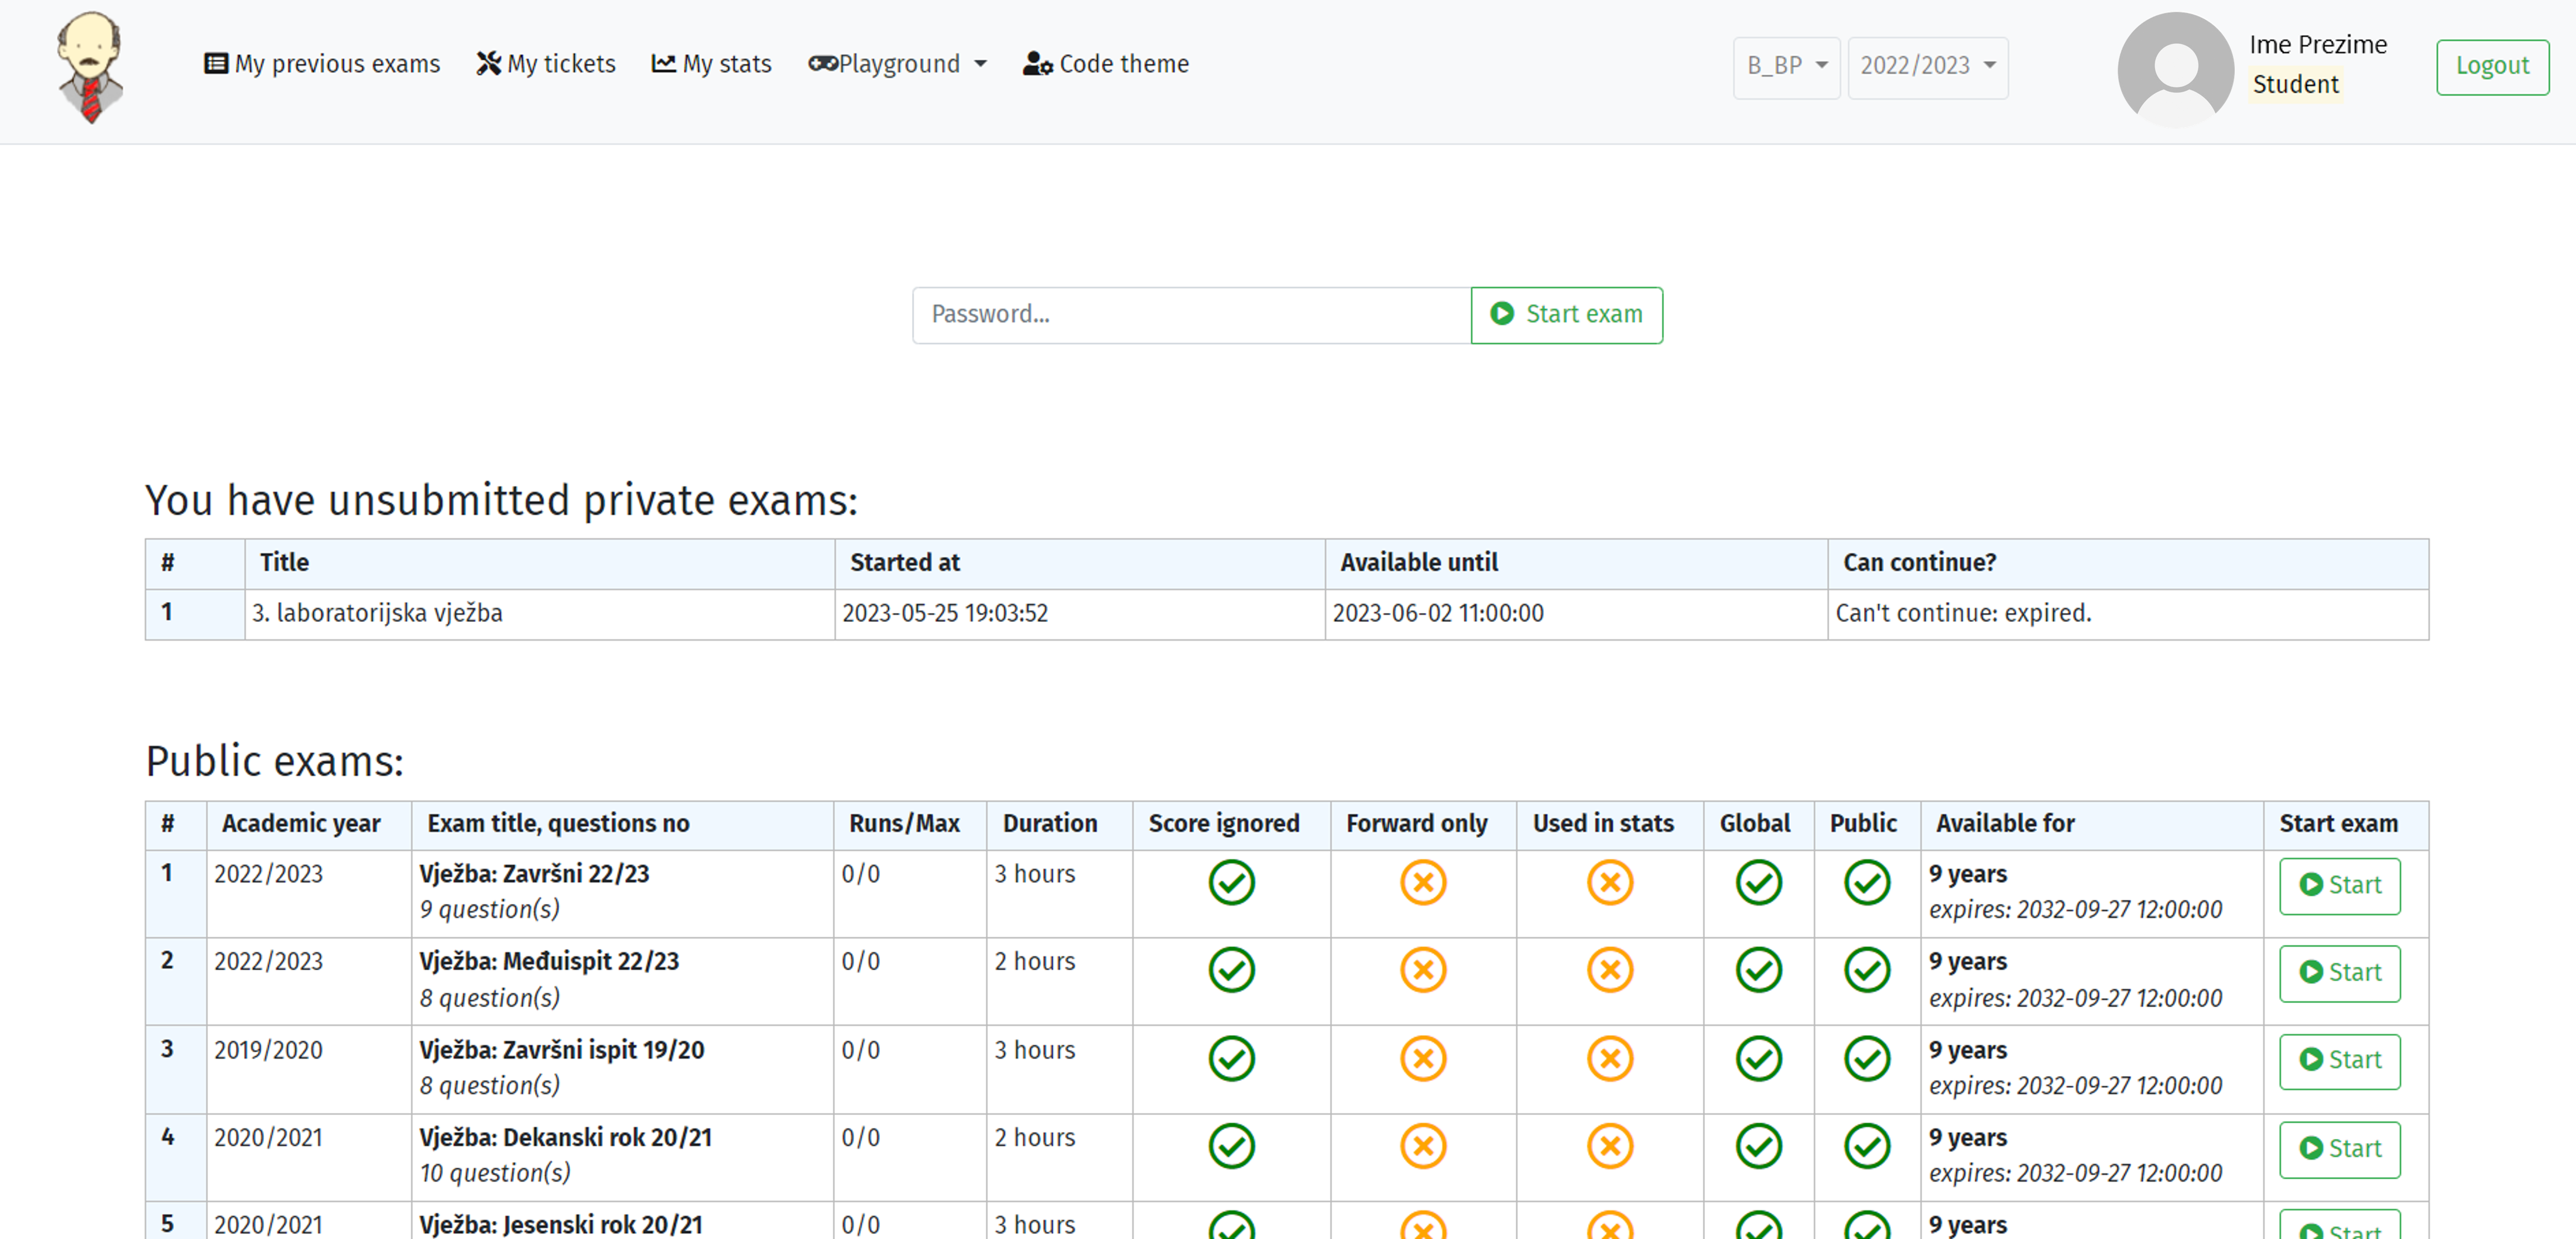
\includegraphics[scale=0.4]{slike/edgar1}
			%veličina slike u odnosu na originalnu datoteku i pozicija slike
			\centering
			\caption{Edgar: početna stranica i popis vježbi za ispite}
			\label{fig:pocstr}
		\end{figure}
				\noindent\\
		Ostale funkcionalnosti BytePita vrlo su slične Edgaru: uloge natjecatelja i studenta su slične, oni mogu učitavati i provjeravati svoj kod, pokrenuti probni ispit (slika \ref{fig:ispit}) (u BytePitu virtualno natjecanje) kao i pristupiti ispitu (odnosno natjecanju). Koncept natjecanja i ispita vrlo je sličan - korisnicima su dostupni svi ispitni zadaci istovremeno, a po završetku se ti zadaci objavljuju na stranici za vježbu. 
		Ono što u BytePitu predstavlja uloga voditelja, u Edgaru je asistent/profesor koji ima ovlasti objavljivanja tj. izrade zadataka i organizaciju ispita (odabir zadataka, trajanja). U Edgaru čak postoji i stranica sa statistikom koja prikazuje uspješnost u odnosu na druge studente, postotak točno riješenih zadataka i sl.(slika  \ref{fig:stats}). BytePit ima stranicu slične namjene, ali ipak s drugačijim podacima: na njoj natjecatelj može vidjeti tuđa rješenja i njihovu uspješnost, kao i svoj rang.	\\
		
		
			%unos slike
	
		
		\begin{figure}[H]
			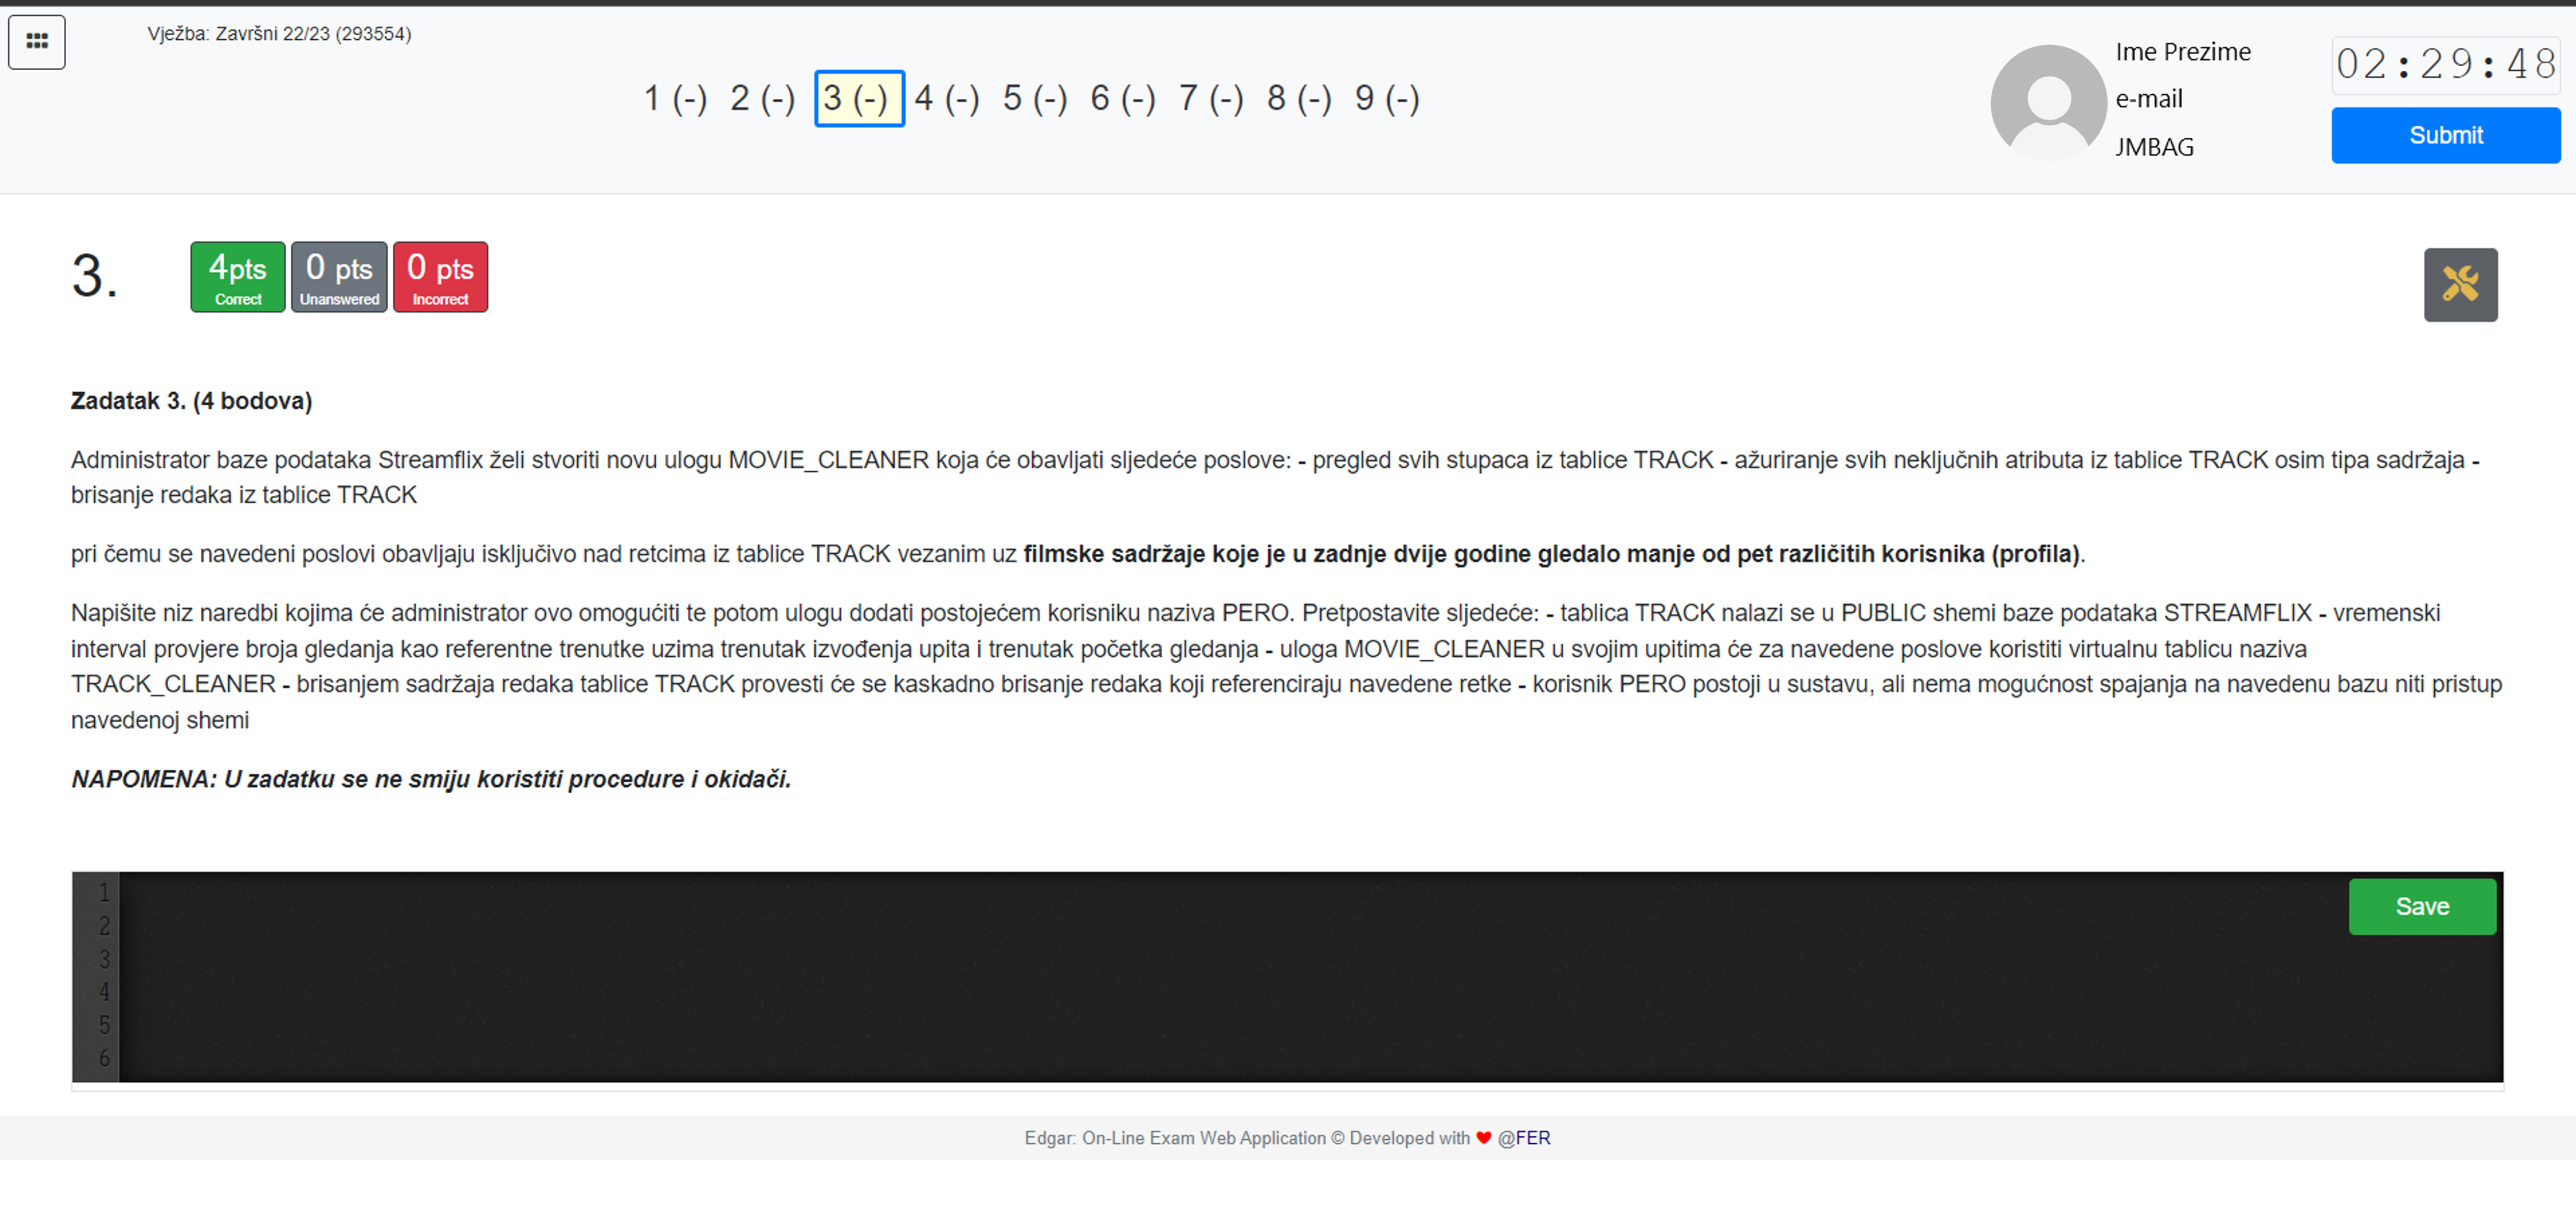
\includegraphics[scale=0.4]{slike/edgar3}
			%veličina slike u odnosu na originalnu datoteku i pozicija slike
			\centering
			\caption{Edgar: probni ispit}
			\label{fig:ispit}
		\end{figure}
		
		\begin{figure}[H]
			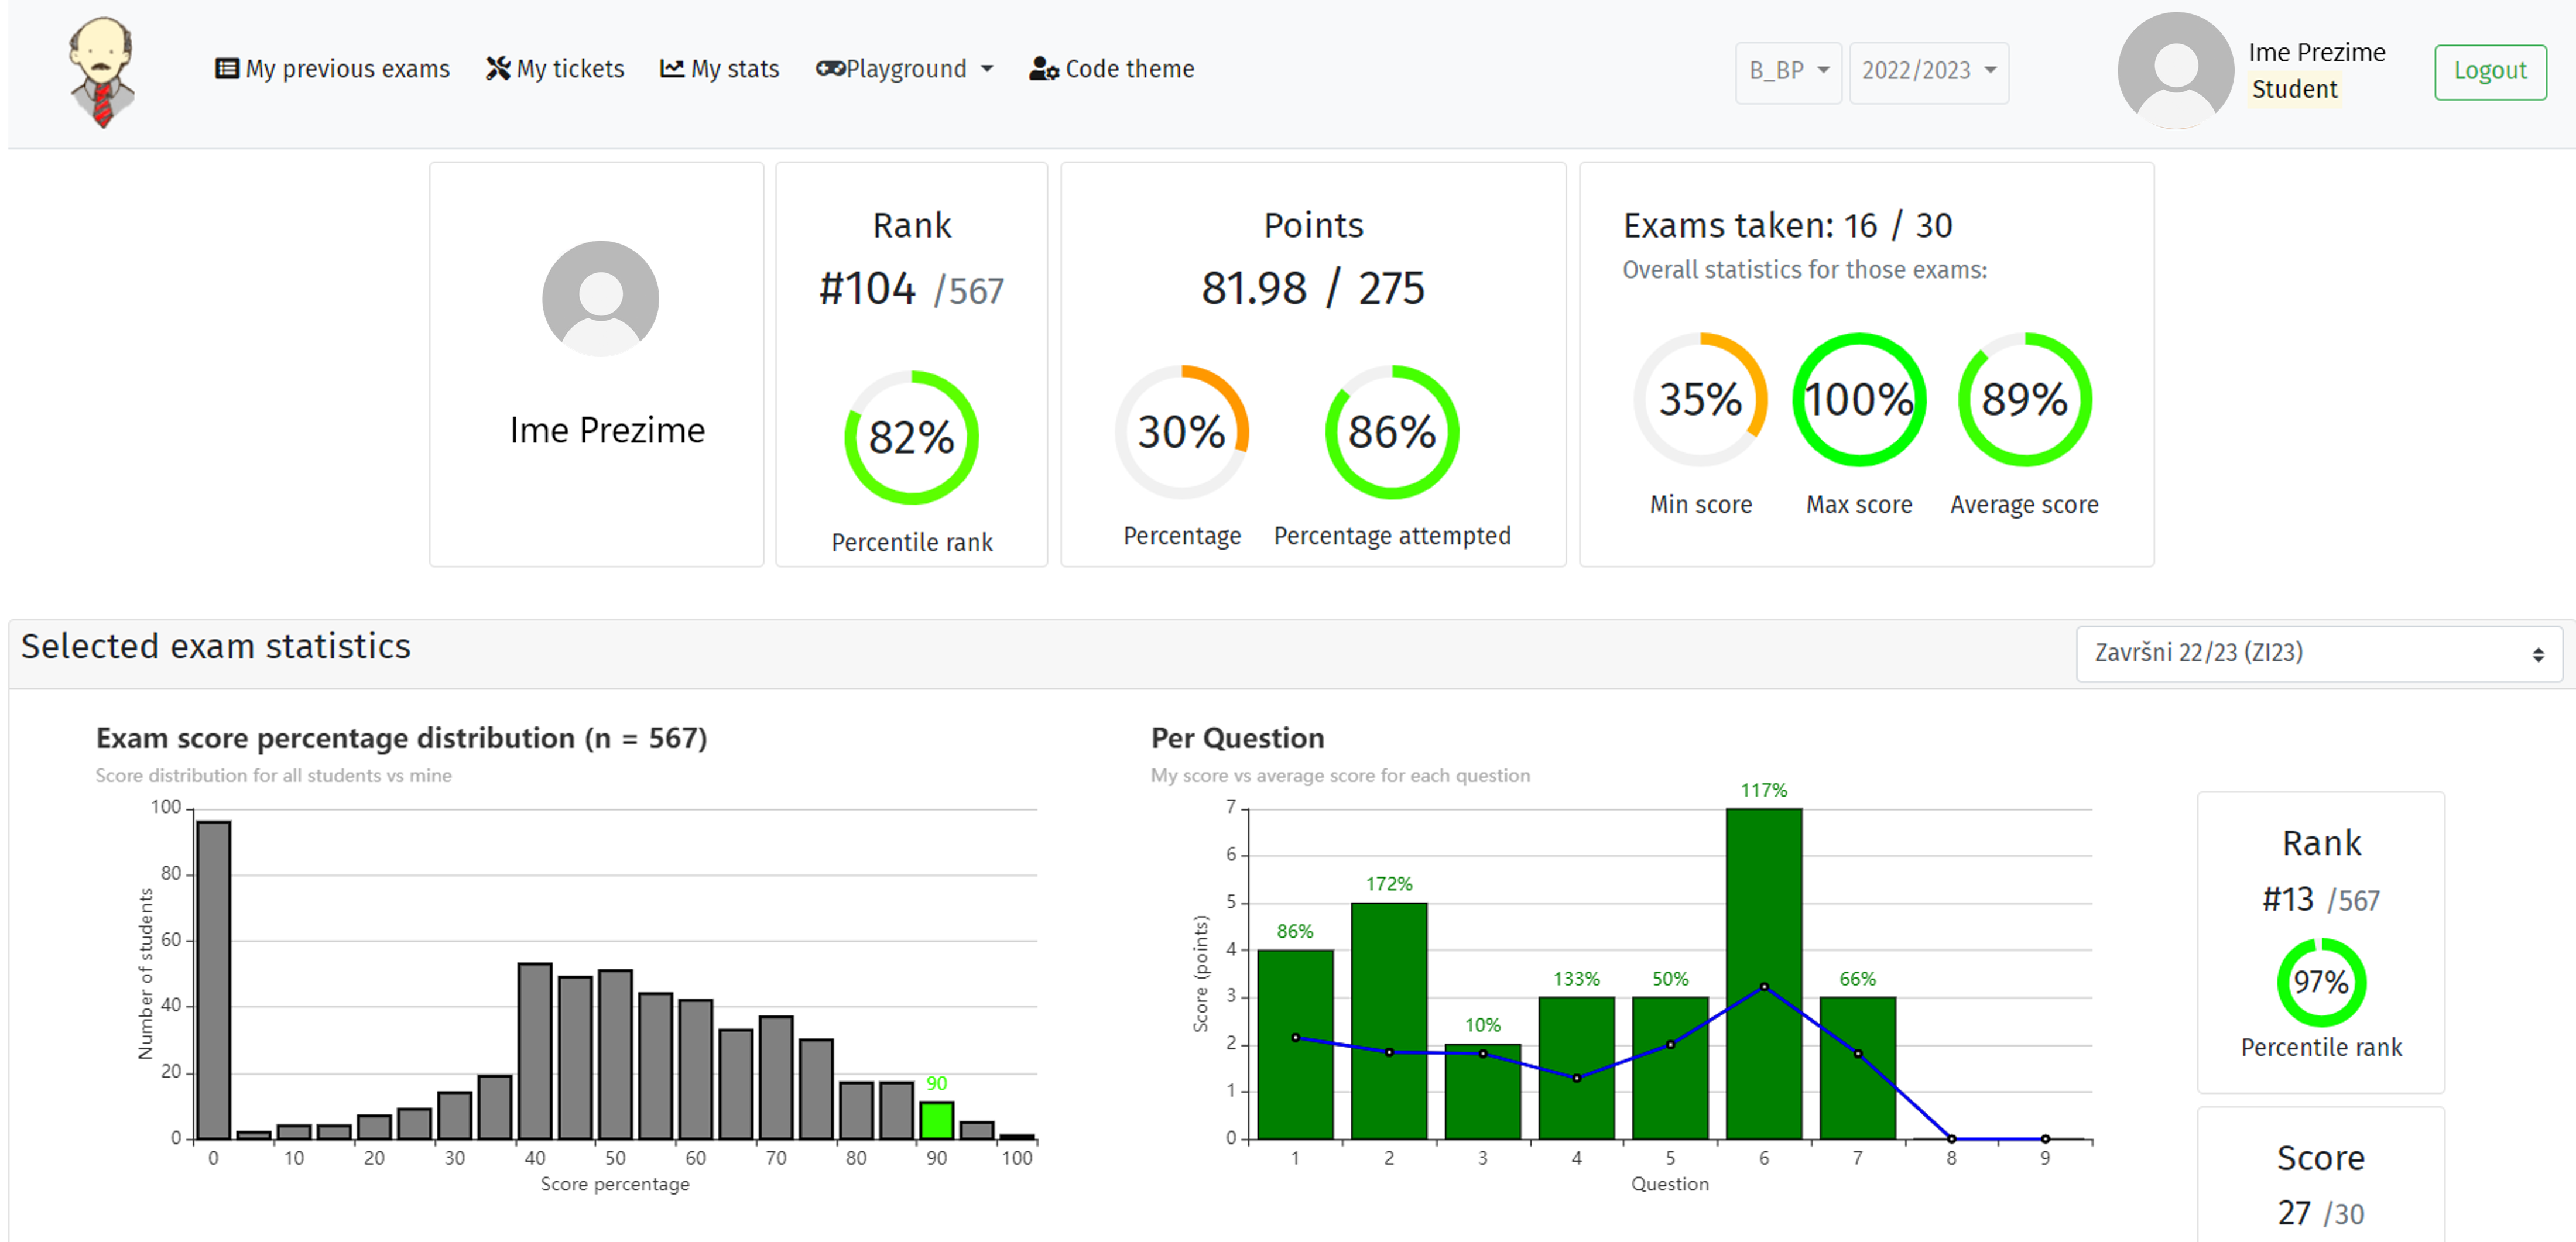
\includegraphics[scale=0.4]{slike/edgar2}
			%veličina slike u odnosu na originalnu datoteku i pozicija slike
			\centering
			\caption{Edgar: stranica sa statistikom}
			\label{fig:stats}
		\end{figure}
		
		\noindent\\
			Osim Edgara, postoji jos niz aplikacija sličnih BytePitu, a jedna od njih je Codeforces, web aplikacija koja omogućuje sudjelovanje u online natjecanjima. Gotovo i da nema razlike među ovim aplikacijama: na profilima korisnika vidljiva je njihova statistika, omogućen je pristup virtualnim natjecanjima koja simuliraju prava, vidljiva je lista problema kao i njihovih rješenja koaje su učitali korisnici (slika \ref{fig:problemi})... Ta rješenja nisu uvijek vidljiva, vidljivost ovisi o postavkama natjecanja tako je da ovisno o sudjelovanju nekim korisnicima onemogućen pregled predanih rješenja. Nasuprot tomu, u BytePitu rješenja može dohvatiti samo natjecatelj koji je i sam točno riješio zadatak. Bitna razlika u ovom je slučaju također i to što Codeforces omogućava svim korisnicima da učitaju zadatke, koji potom prolaze dodatne provjere da bi se utvrdila njihova ispravnost, dok je u BytePitu ta mogućnost otvorena samo voditeljima, i to bez dodatnih provjera nakon objave zadatka. Na profilima korisnika koji su zadatke učitali ti zadaci nisu vidljivi (u BytePitu se oni nalaze na profilima voditelja).
		Slično kao u našoj aplikaciji, nakon natjecanja moguće je na profilima korisnika vidjeti njihova rješenja i rezultate testova ali čak i bez registracije: svaki korisnik vidi rješenja svakog korisnika te nije potrebna registracija. Ono što registracija omogućuje je, dakako, sudjelovanje u natjecanjima i vritualnim natjecanjima te izvršavanje i predaja koda za riješene zadatake za vježbu (slika \ref{fig:run}) (neregistrirani korisnik može vidjeti tekst zadatka, ali ne moze izvršiti kod i time provjeriti točnost rješenja). Ono što BytePit omogućuje, a Codeforces ne je mogućnost virtualnog natjecanja koje se sastoji od nasumičnih zadataka: u potonjem se nude samo replike stvarnih natjecanja koje se mogu pokrenuti. \\
		
			\begin{figure}[H]
			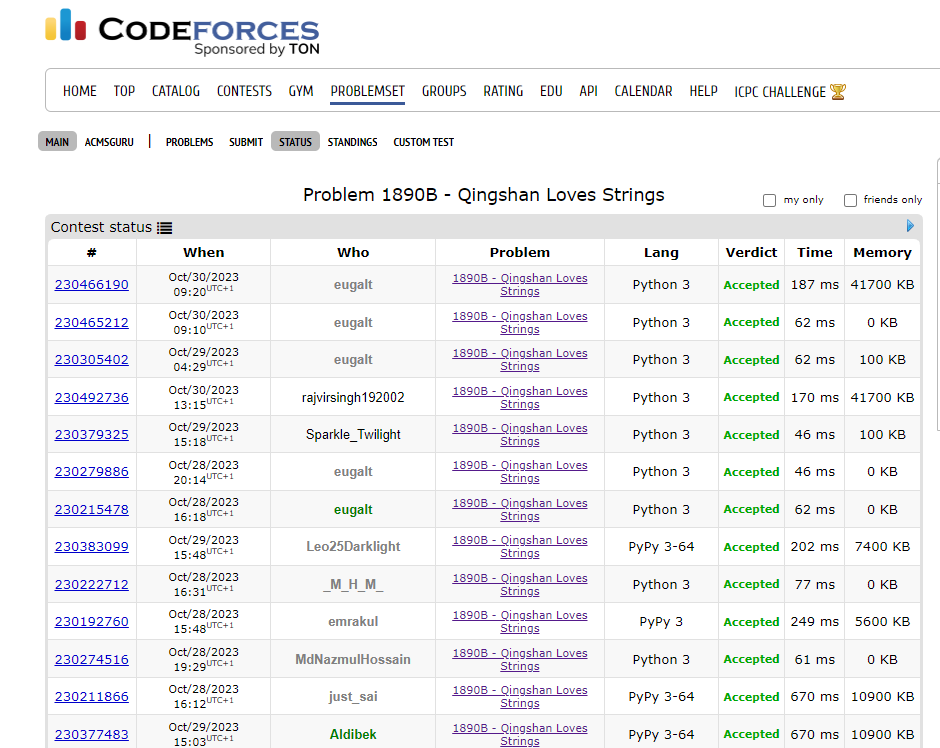
\includegraphics[scale=0.4]{slike/cf1}
			%veličina slike u odnosu na originalnu datoteku i pozicija slike
			\centering
			\caption{Codeforces: rješenja različitih korisnika}
			\label{fig:problemi}
		\end{figure}
		
		\begin{figure}[H]
			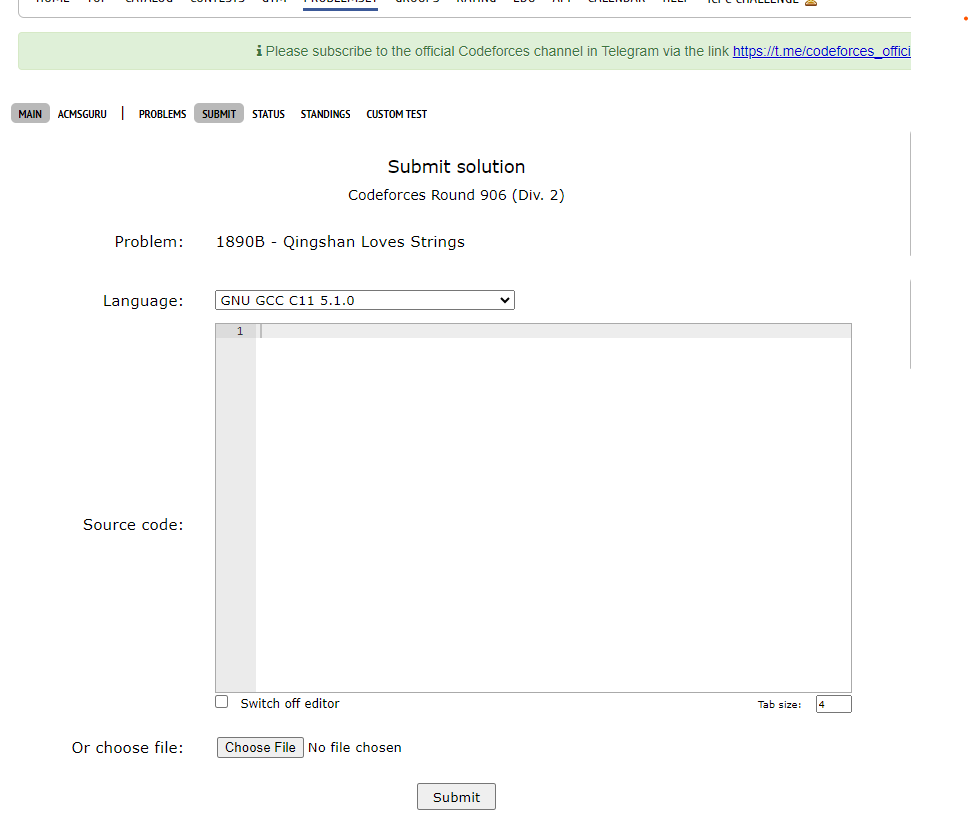
\includegraphics[scale=0.4]{slike/cf2}
			%veličina slike u odnosu na originalnu datoteku i pozicija slike
			\centering
			\caption{Codeforces: mogućnost izvršavanja koda}
			\label{fig:run}
		\end{figure}
		
		\noindent\\
		BytePit je aplikacija koja svakako može imati širu primjenu od ovdje opisane: dok je trenutna verzija aplikacije pogodna uglavnom za programerska natjecanja, s manjim preinakama ona bi se mogla koristiti u razne svrhe. Svakako bi bila dobra ideja koristiti aplikaciju kao svojevrsni test pri zapošljavanju programera odnosno za selekciju najboljih kandidata: kandidati bi dobili podatke za pristup i od njih bi se tražilo da riješe određen broj zadataka (naravno, drugačije vrste od natjecateljskih). Tako bi se lakše probralo bolje kandidate koji ulaze u uži izbor za određenu poziciju. Prilagodbom težine zadataka, BytePit bi mogao postati i platforma za vježbu i učenje programiranja. Naravno, u tom bi slučaju bilo potrebno osmisliti i kratke tečajeve programiranja, kao što to postoji na npr. Codecademy-u.
		Aplikacija bi se mogla proširiti i na način da bude slična gore predstavljenoj aplikaciji Edgar: mogla bi biti platforma za ispite iz programiranja, kako na fakultetu, tako i u osnovnim i srednjim školama.\\
		
		\eject

		
		
		\section{Primjeri u \LaTeX u}
		
		\textit{Ovo potpoglavlje izbrisati.}\\

		U nastavku se nalaze različiti primjeri kako koristiti osnovne funkcionalnosti \LaTeX a koje su potrebne za izradu dokumentacije. Za dodatnu pomoć obratiti se asistentu na projektu ili potražiti upute na sljedećim web sjedištima:
		\begin{itemize}
			\item Upute za izradu diplomskog rada u \LaTeX u - \url{https://www.fer.unizg.hr/_download/repository/LaTeX-upute.pdf}
			\item \LaTeX\ projekt - \url{https://www.latex-project.org/help/}
			\item StackExchange za Tex - \url{https://tex.stackexchange.com/}\\
		
		\end{itemize} 	


		
		\noindent \underbar{podcrtani tekst}, \textbf{podebljani tekst}, 	\textit{nagnuti tekst}\\
		\noindent \normalsize primjer \large primjer \Large primjer \LARGE {primjer} \huge {primjer} \Huge primjer \normalsize
				
		\begin{packed_item}
			
			\item  primjer
			\item  primjer
			\item  primjer
			\item[] \begin{packed_enum}
				\item primjer
				\item[] \begin{packed_enum}
					\item[1.a] primjer
					\item[b] primjer
				\end{packed_enum}
				\item primjer
			\end{packed_enum}
			
		\end{packed_item}
		
		\noindent primjer url-a: \url{https://www.fer.unizg.hr/predmet/proinz/projekt}
		
		\noindent posebni znakovi: \# \$ \% \& \{ \} \_ 
		$|$ $<$ $>$ 
		\^{} 
		\~{} 
		$\backslash$ 
		
		
		\begin{longtblr}[
			label=none,
			entry=none
			]{
				width = \textwidth,
				colspec={|X[8,l]|X[8, l]|X[16, l]|}, 
				rowhead = 1,
			} %definicija širine tablice, širine stupaca, poravnanje i broja redaka naslova tablice
			\hline \SetCell[c=3]{c}{\textbf{naslov unutar tablice}}	 \\ \hline[3pt]
			\SetCell{LightGreen}IDKorisnik & INT	&  	Lorem ipsum dolor sit amet, consectetur adipiscing elit, sed do eiusmod  	\\ \hline
			korisnickoIme	& VARCHAR &   	\\ \hline 
			email & VARCHAR &   \\ \hline 
			ime & VARCHAR	&  		\\ \hline 
			\SetCell{LightBlue} primjer	& VARCHAR &   	\\ \hline 
		\end{longtblr}
		

		\begin{longtblr}[
				caption = {Naslov s referencom izvan tablice},
				entry = {Short Caption},
			]{
				width = \textwidth, 
				colspec = {|X[8,l]|X[8,l]|X[16,l]|}, 
				rowhead = 1,
			}
			\hline
			\SetCell{LightGreen}IDKorisnik & INT	&  	Lorem ipsum dolor sit amet, consectetur adipiscing elit, sed do eiusmod  	\\ \hline
			korisnickoIme	& VARCHAR &   	\\ \hline 
			email & VARCHAR &   \\ \hline 
			ime & VARCHAR	&  		\\ \hline 
			\SetCell{LightBlue} primjer	& VARCHAR &   	\\ \hline 
		\end{longtblr}
	


		
		
		%unos slike
		\begin{figure}[H]
			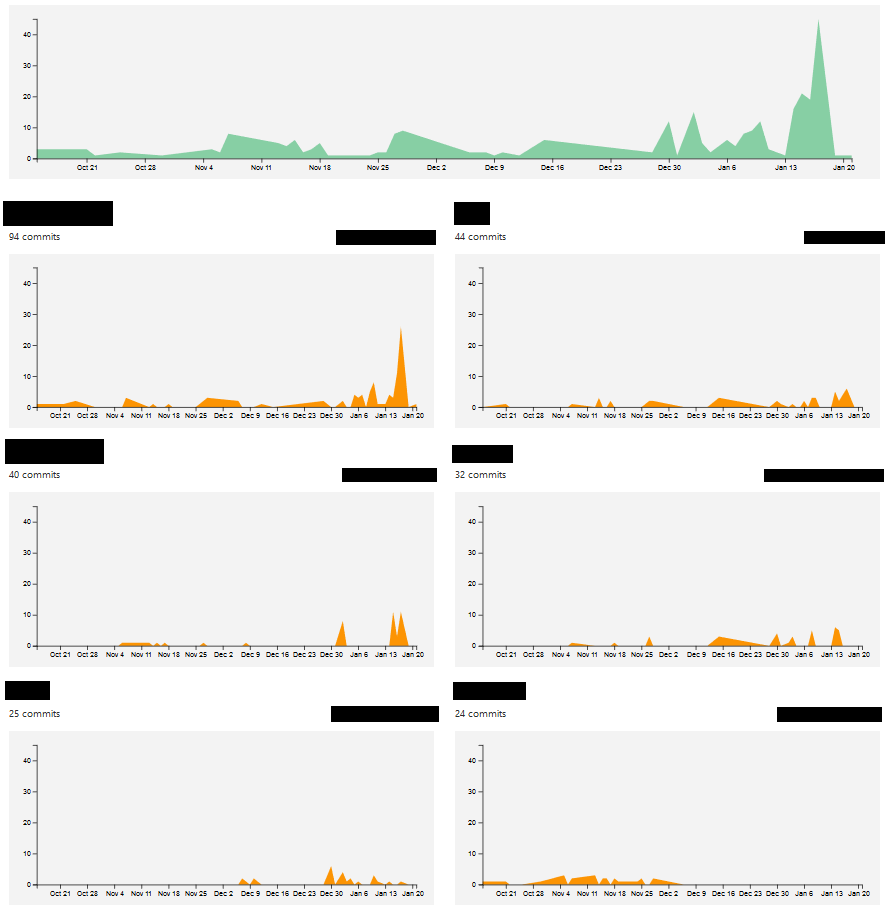
\includegraphics[scale=0.4]{slike/aktivnost.PNG} %veličina slike u odnosu na originalnu datoteku i pozicija slike
			\centering
			\caption{Primjer slike s potpisom}
			\label{fig:promjene}
		\end{figure}
		
		\begin{figure}[H]
			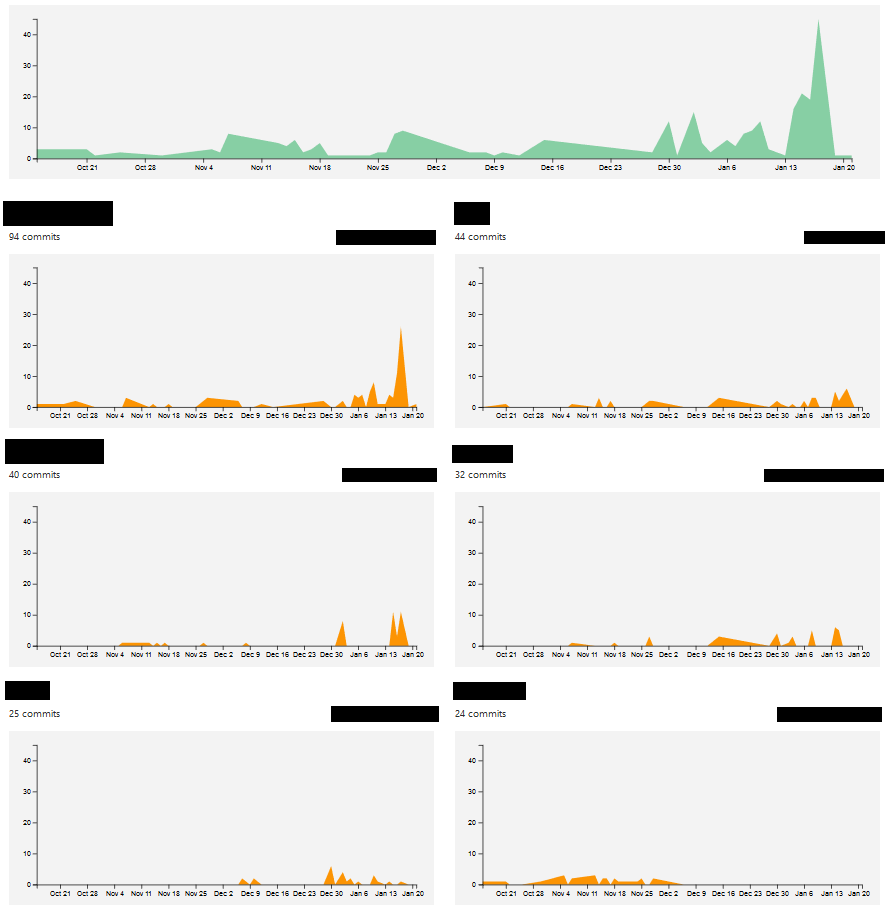
\includegraphics[width=\textwidth]{slike/aktivnost.PNG} %veličina u odnosu na širinu linije
			\caption{Primjer slike s potpisom 2}
			\label{fig:promjene2} %label mora biti drugaciji za svaku sliku
		\end{figure}
		
		Referenciranje slike \ref{fig:promjene2} u tekstu.
		
		\eject
		
	